\subsection{Read thermistor values with ADC}
The ADC is a component of the SCA that is used to convert the analog signal of the thermistors to a digital signal that can be read by the computer. To measure the voltage across any thermistor connected to the ADC, first the current source must be switched on for that channel, and then a read command must be issued. The figures below show the GBT client ADC tab with the required parameters. It is important to note that \textbf{Version} must be set to \textbf{2}, \textbf{Address} must be set to the desired command, and \textbf{Line} must be set to the desired channel to be probed. 


\begin{figure}[ht]
      \centering
  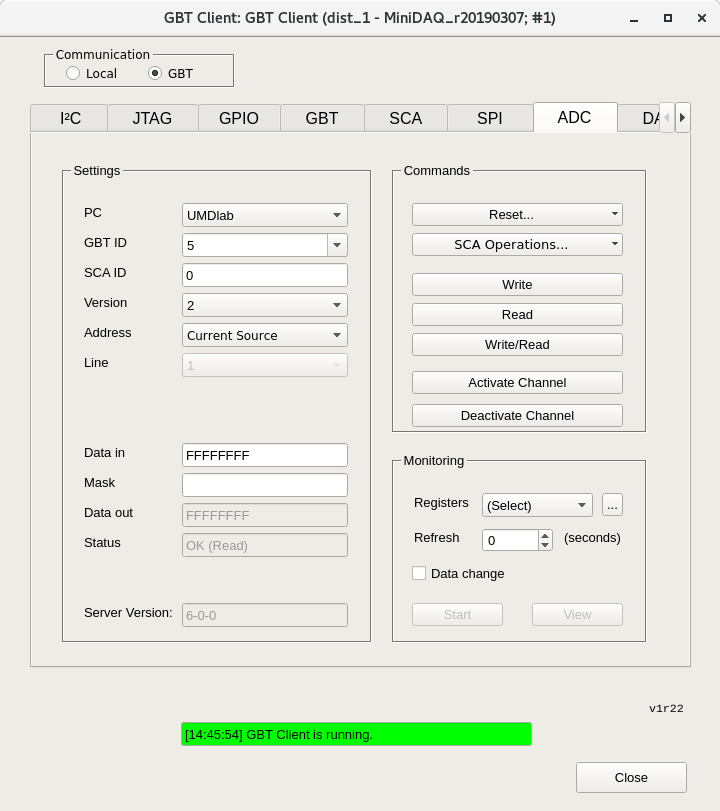
\includegraphics[width=0.9\textwidth]{res/gbt_client_adc_readout_currentsource.png}
      \caption{Parameters to send a command to the SCA to activate 100 microamp current sources for specific channels.}
      \label{fig:gbt-file}

\begin{lstlisting}
  | ADC Channel | Signal Name | Line | Current Source Register Setting |
  | CH 00 | DC_PLAT_RTD_A | 0 | N/A
  | CH 01 | OM45_THERM_Leg_A | 1 | 0x02000000 |
  | CH 16 | OM23_THERM_Leg_A | 16 | 0x00000100 |
  | CH 17 | OM61_THERM_Leg_A | 17 | 0x00000200 |
  | CH 18 | OMMC_THERM_Leg_A | 18 | 0x00000400 |
  | CH 31 | Internal SCA Therm | ??? | ??? |

  It is normal operation to open every single current source on every channel by setting \texttt{Current Source} 
  to \texttt{0xFFFFFFFF} instead of having only one channel with current. This has been approved by SCA experts.
\end{lstlisting}


\begin{figure}[ht]
      \centering
  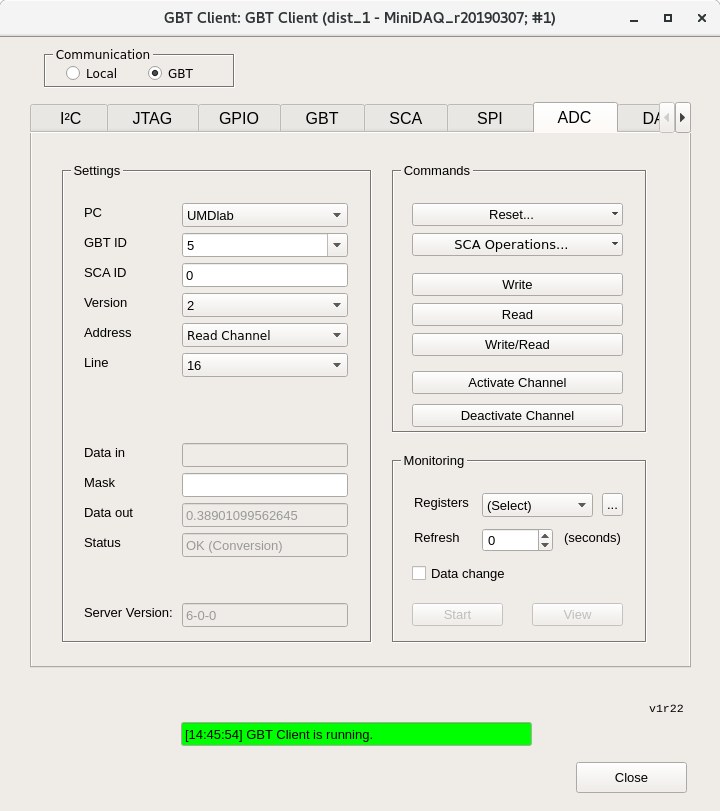
\includegraphics[width=0.9\textwidth]{res/gbt_client_adc_readout_readchannel.png}
      \caption{Parameters to send a command to the SCA to read the voltage on the channel specified by the given line}
      \label{fig:gbt-file}
